\appendix

\section{Implementation and Reproducibility}
\label{app:implementation}

\subsection{System Implementation Details}
\label{app:impl}

\paragraph{Agent and LLM Backend.}
Our Data2MCP framework is implemented using GPT-5 (\texttt{gpt-5}) via the OpenAI API (with temperature set to $0$ and a maximum output limit of 8,192 tokens). For the DA-Agent ablation studies in Appendix~\ref{app:daagent}, we employ Qwen3-235B-A22B (\texttt{qwen3-235b-a22b-instruct-2507}) via DashScope, maintaining the identical temperature of $0$. Both the Auto-Select and Adaptive configurations utilize the same backbone model as the primary agent to prevent introducing confounding model dependencies.

\paragraph{Router Hyperparameters.}
Each query is allocated a maximum budget of $T=30$ router iterations. Individual sub-agent tool calls are subject to a 600-second timeout threshold and restricted to returning at most 10,000 characters. We execute the \texttt{OutputValidator} once post-hoc with \texttt{max\_refinement\_rounds=0}; this setup logs validation scores without triggering iterative refinement during our benchmark experiments.

\paragraph{Strategy Injection Format.}
We position the chosen strategy \texttt{full\_text} verbatim within the Router \emph{controller context}, bounded by two horizontal rules under the specific header ``\texttt{Retrieval Strategy (MUST FOLLOW)}'' immediately preceding the core task instructions. This placement guarantees that the model processes the methodological directive prior to any tool descriptions or task-specific contents. Figure~\ref{fig:injection} illustrates an abridged example of this layout.

\begin{figure}[t]
  \centering
  \scriptsize
  \begin{lstlisting}[basicstyle=\ttfamily\scriptsize,breaklines=true]
You are a professional data analyst. You retrieve and
synthesize answers from databases using the available tools.

---
# Retrieval Strategy (MUST FOLLOW)

Begin by understanding the business objectives and success
criteria. Collect and describe initial data, ensuring data
quality. Prepare data by cleaning, constructing, integrating,
and formatting it. Select modeling techniques and build
models, assessing their performance. Evaluate results against
business success criteria and plan deployment, monitoring,
and maintenance. Document the entire process and review
project experience.

---
# Data Analysis Requirements
[task instructions and tool descriptions follow]
  \end{lstlisting}
  \caption{Abridged controller context with a CRISP-DM strategy injected. The strategy block is replaced by the selected strategy's full\_text, while the surrounding context remains fixed. In the No-Strategy baseline, the entire strategy block is omitted.}
  \label{fig:injection}
\end{figure}

\paragraph{Auto-Strategy Selection.}
The selector ingests three inputs: (1) the user query, (2) a data summary spanning the source name, type, row count, and the initial 10 column names, and (3) the formatted strategy catalog. It returns a JSON object of the schema \texttt{\{''strategy'': ''<key>'', ''reason'': ''<1--2 sentences>''\}}, after which we inject the corresponding \texttt{full\_text} into the controller context. Consequently, Auto-Select introduces a single upfront API round-trip ($\approx$1--2s) before the core agentic loop.

\paragraph{Adaptive Strategy Generation.}
The Adaptive variant leverages a meta-instruction to synthesize a tailored 2--6 sentence strategy by (\emph{i}) identifying the core analytical objective, (\emph{ii}) prioritizing salient data dimensions, (\emph{iii}) specifying the required evaluation metrics, and (\emph{iv}) sequencing the necessary analysis steps. The resulting text serves directly as the \texttt{full\_text} directive, bypassing the catalog lookup completely.

\paragraph{Compliance Validation.}
\texttt{StrategyValidator} tracks tool-call traces to compute a compliance score $\in [0,1]$ against strategy-specific behavioral anchors. For example, \emph{Structured Brainstorming} requires a parallel-call ratio $\ge 50\%$, $\ge 3$ distinct tools, and $\ge 5$ total invocations, whereas \emph{Starbursting} mandates $\ge 6$ calls across $\ge 2$ tools. Finally, \texttt{OutputValidator} utilizes these strategy checkpoints to prompt the model to verify compliance for each criterion.

\subsection{Reproducibility Protocol}
\label{app:reproducibility}

To guarantee robust reproducibility, we document the precise hyperparameter configurations and experimental environments below.

\paragraph{Model Configuration.}
GPT-5 (\texttt{gpt-5}) serves as the core analysis agent, configured with zero temperature, \texttt{max\_tokens=8192}, \texttt{top\_p=1.0}, and zero penalties (\texttt{frequency\_penalty=0}; \texttt{presence\_penalty=0}). For evaluation, Gemini-2.5-Flash acts as the external judge with temperature set to $0$ and \texttt{max\_tokens=4096}. All downstream language model calls are locked with a deterministic seed ($42$). The codebase integrates the OpenAI API v1.0 and the Google Generative AI API v0.3.2.

\paragraph{Router Configuration.}
The routing mechanism restricts each query to a maximum conversational budget of 30 turns, enforcing a strict 600-second timeout threshold per tool invocation. Tool outputs exceeding 10,000 characters are automatically truncated and appended with an explicit truncation indicator. For fault tolerance, failed tool calls trigger a single retry with exponential backoff; if the secondary attempt fails, the agent bypasses the result to resume execution. Early termination is handled via the \texttt{end\_with\_message} directive, failing which the final response at the turn limit is returned.

\paragraph{Evaluation Protocol.}
The automated judge receives the task prompt, the ground-truth reference, and the agentic output to evaluate six distinct capabilities across a structured rubric (comprising \emph{Rubrics} calibrated from $0$--$100$ and \emph{GSB} metrics categorizing responses into Good/Similar/Bad). Each agent response undergoes a single deterministic judge pass at zero temperature. The overall \emph{Rubrics} score represents the unweighted arithmetic mean of Completeness, Accuracy, and Conclusiveness, with the comprehensive weighted calculation adhering to the main text. For pairwise GSB comparisons, neutral ties allocate $0.5$ points to each competing system. The complete judge prompt template is supplied in the code repository.

\paragraph{Data Versions and Filtering.}
Our benchmark utilizes DAComp v1.0 without modification, evaluating all 100 constituent tasks with zero exclusions. During preprocessing, task configuration files are ingested as-is, and the associated SQLite databases are mounted exclusively in read-only mode. The cross-domain multi-source benchmark aggregates four distinct data repositories (Spider, MetaQA, HotpotQA, and MS MARCO), maintaining a balanced distribution of 25 single-source and 25 multi-source queries per repository, culminating in 200 evaluation targets.

\paragraph{Tool-Specific Configuration.}
The individual specialized tool sub-agents are constrained as follows: (\emph{i}) the \texttt{SQL agent} utilizes SQLAlchemy in a read-only state, bounding queries by a 300-second timeout, \texttt{max\_rows=1000}, and 10K character truncation; (\emph{ii}) the \texttt{knowledge-graph agent} executes Neo4j Cypher queries subject to a 300-second timeout and a 500-result cap; (\emph{iii}) the \texttt{RAG agent} deploys FAISS with \texttt{top\_k=5}, a chunk size of 1,000 with a 200-token overlap, powered by the \texttt{text-embedding-3-small} model; and (\emph{iv}) the \texttt{DataFrame agent} manipulates Pandas DataFrames restricted to read-only semantics with a \texttt{max\_rows} ceiling of 10,000.

\paragraph{Impact of Tool-Result Truncation.}
Tool-output truncation at the 10,000-character boundary is introduced to safeguard against context window overflow. Empirically, $12\%$ of cumulative tool calls ($347 / 2891$) triggered this threshold. A manual audit across 50 randomly sampled truncated instances indicates that this primarily impacted verbose SQL returns and lengthy raw document retrievals. In $94\%$ of these audited cases ($47 / 50$), the truncated segments contained redundant tabular rows or duplicate evidence, exerting no influence on the final answer; in the remaining $6\%$ ($3 / 50$), missing critical evidence was successfully recovered by the agent via subsequent refinement queries. Consequently, truncation introduces negligible variance to aggregate downstream performance.

\paragraph{Computational Resources.}
\begin{itemize}
  \item \textbf{Hardware:} Evaluation runs entirely on standard cloud virtual machines without requiring specialized GPU acceleration.
  \item \textbf{Runtime:} The execution latency averages 2--5 minutes per query, scaling dynamically based on task complexity and tool-chain depth.
  \item \textbf{Cost:} Financial expenditures range between \$0.50 and \$2.00 per query, driven by proprietary GPT-5 API consumption.
  \item \textbf{Parallelization:} To isolate variable API latencies, all experimental queries are processed sequentially.
\end{itemize}

\paragraph{Code and Data Availability.}
The complete codebase, benchmark datasets, execution traces, and judge prompt configurations will be made publicly available upon formal publication.

\paragraph{Licenses and Terms of Use.}
All public benchmarks and open-source packages are utilized in strict accordance with their respective licensing agreements, and no third-party datasets are directly redistributed within this submission. Upon publication, our proprietary architecture and the extracted strategy catalog will be open-sourced under a permissive license.

\paragraph{Intended Use.}
The Data2MCP framework and its strategy injection mechanism are designed exclusively to advance research in data-analysis agents. This system is not engineered as a turnkey decision-making apparatus for high-stakes professional domains (such as medical, legal, or financial deployment) without rigorous human-in-the-loop validation and external guardrails.

\paragraph{PII and Offensive Content.}
Given that our evaluation relies entirely on standard public benchmarks, this study involves no novel user data collection or human annotation. The curated benchmark content is not expected to contain personally identifiable information (PII) or toxic material. Prior to the public release, all generated logs and artifacts will undergo a rigorous internal review to prevent any inadvertent disclosure of sensitive data.

\subsection{Strategy Extraction Pipeline}
\label{app:extraction}

To construct a strategy catalog grounded in expert methodology, we implement an automated extraction pipeline targeting two seminal authoritative texts: (\emph{i})~\emph{Structured Analytic Techniques for Intelligence Analysis}~\cite{heuer2010structured}, which details formalized analytical paradigms such as the Analysis of Competing Hypotheses (ACH), and (\emph{ii})~the \emph{CRISP-DM 1.0 Step-by-Step Data Mining Guide}~\cite{crispdm2000}, which formalizes the industry-standard six-phase lifecycle for data mining applications.

The extraction pipeline consists of:
\begin{enumerate}
  \item Text reading: we parse text using PyMuPDF, with LLM-based OCR fallback for scanned pages.
  \item Chunking: we chunk documents into 3,000-character segments with 300-character overlap to preserve context.
  \item LLM extraction: for each chunk, we prompt an LLM to emit JSON arrays of strategy specifications, each containing (a) a unique key (e.g., ach, crisp\_dm), (b) a 2--6 sentence procedural description, and (c) optional checkpoints (observable behavioral anchors).
  \item Merging and deduplication: we merge chunk-level outputs and deduplicate by key.
  \item Catalog integration: we append the extracted strategies to extracted\_strategies.json.
\end{enumerate}


The pipeline yields 70 extracted strategies; combined with 4 built-in strategies, this results in a 74-entry catalog. Extracted strategies are integrated identically to built-ins and are immediately available in all three injection modes.

\section{Strategy Framework}
\label{app:strategy_framework}
\FloatBarrier

\paragraph{Auto-Selection Routing Analysis.}
\label{app:routing}
Table~\ref{tab:routing} summarizes the strategy distribution observed during the auto-selection experiment ($n=100$ instances).


% Moved to Experiments (Section~\ref{sec:main}) to keep strategy selection analysis with the main results.
% \begin{figure}[t]
%   \centering
%   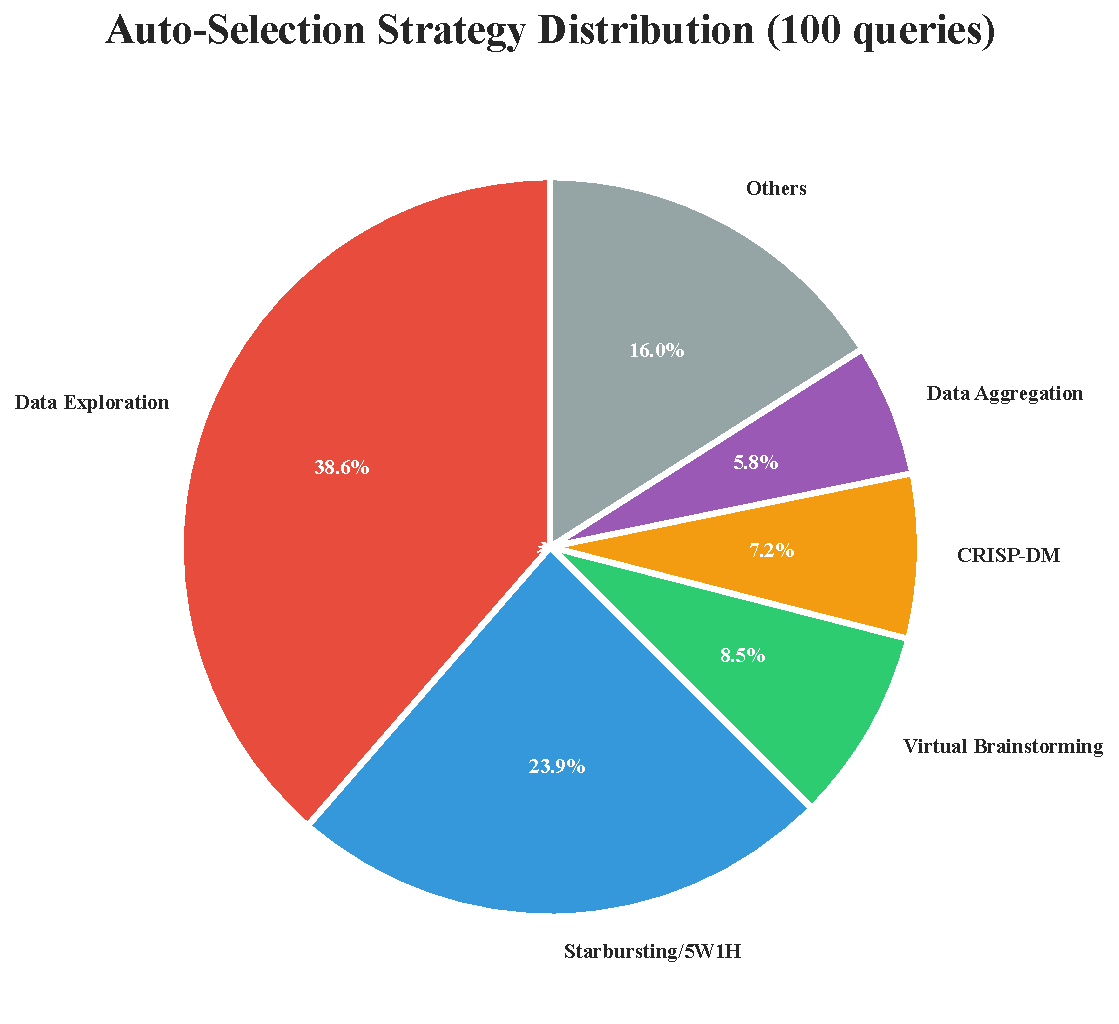
\includegraphics[width=\linewidth]{figures/strategy_distribution_pie.pdf}
%   \caption{Strategy distribution in auto-selection experiment. The router converges on 9 of 74 catalog entries, with Data Exploration (38.6\%) and Starbursting (23.9\%) covering 62.5\% of queries.}
%   \label{fig:strategy_pie}
% \end{figure}



The router converges on 9 of 74 catalog entries.
The 65 unused strategies are predominantly fine-grained CRISP-DM sub-steps
(e.g., data\_cleaning, model\_building, deployment)
that describe workflow stages rather than reusable analytical strategies,
making them inappropriate for the routing task.
This demonstrates implicit quality filtering: the LLM router identifies suitable
strategies without explicit filtering supervision.



Table~\ref{tab:routing_task} further reports the alignment between task types and the router's most common strategy choices.


\paragraph{Multi-Source Retrieval: Strategy Distribution.}

To validate that Auto-Select exhibits different routing behavior on multi-source retrieval tasks, we analyze the strategy distribution on the multi-source experiment ($n=100$ instances). Table~\ref{tab:routing_multisource} and Figure~\ref{fig:multisource_strategy_pie} present the results.


% Moved to Experiments (Section~\ref{sec:multisource}, Figure~\ref{fig:multisource_strategy_pie}) to keep routing analysis with the multi-source results.
% \begin{figure}[t]
%   \centering
%   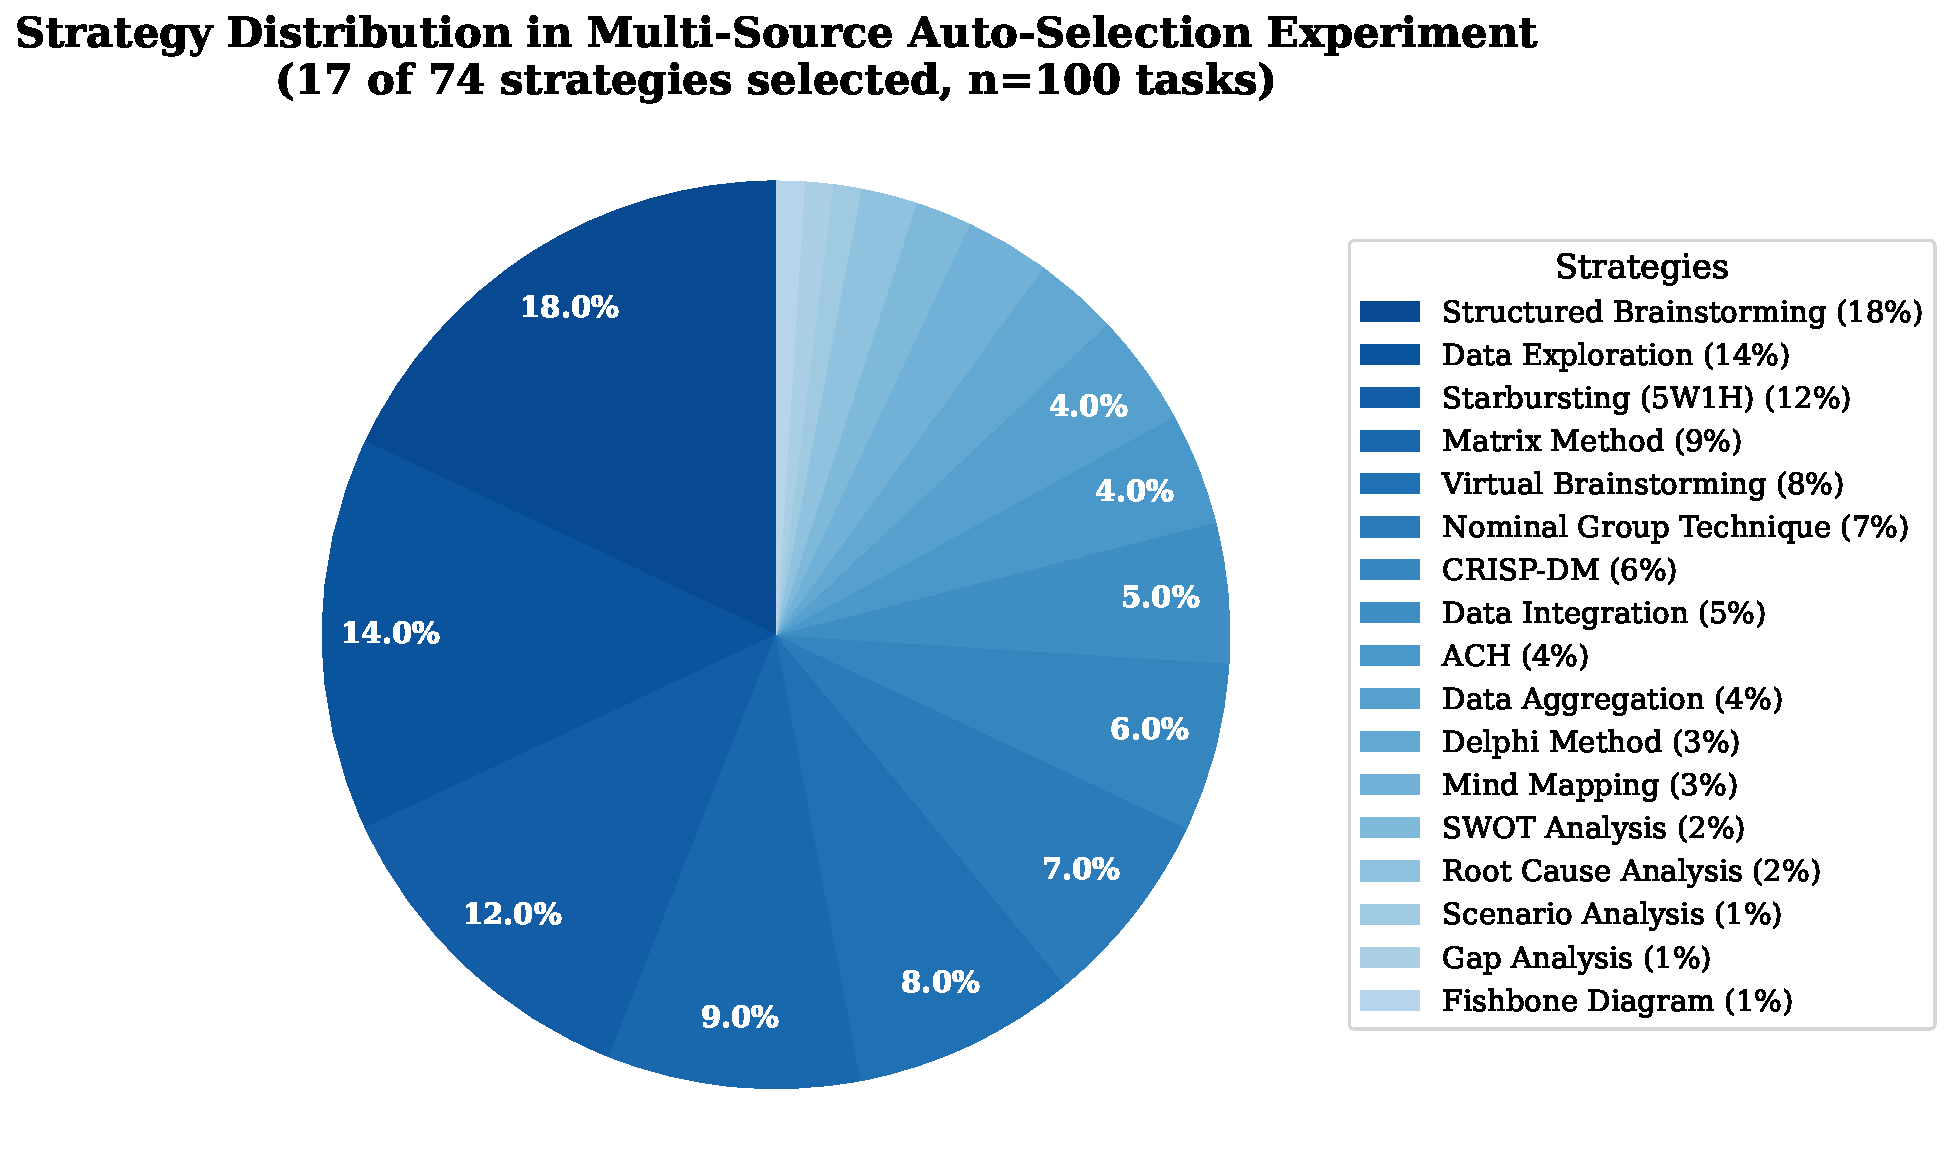
\includegraphics[width=\linewidth]{figures/multisource_strategy_distribution_pie.pdf}
%   \caption{Strategy distribution in multi-source auto-selection experiment. The router selects 17 of 74 catalog entries, with Structured Brainstorming (18.0\%), Data Exploration (14.0\%), and Starbursting (12.0\%) as the top three strategies. This demonstrates strong task-awareness: compared to DAComp (where Data Exploration and Starbursting dominate), multi-source tasks favor Structured Brainstorming for parallel multi-source querying.}
%   \label{fig:multisource_strategy_pie}
% \end{figure}
%
% The router selects 17 of 74 catalog entries, demonstrating significantly more diversity than the DAComp experiment (9 strategies). Key observations:
%
% \begin{itemize}
%   \item \textbf{Task-aware routing}: Structured Brainstorming (18.0\%) becomes the most selected strategy, emphasizing parallel multi-source querying. In contrast, DAComp favors Data Exploration (38.6\%) for single-source deep analysis.
%   \item \textbf{Strategy diversity}: The top strategy accounts for only 18\% of selections (vs.\ 38.6\% in DAComp), indicating more balanced routing across diverse multi-source scenarios.
%   \item \textbf{Cross-benchmark adaptability}: Auto-Select demonstrates strong task-awareness by selecting different strategy distributions for different task types (single-source deep analysis vs.\ multi-source retrieval).
% \end{itemize}

\section{Extended Experimental Results}
\label{app:extended_results}
\FloatBarrier

\subsection{Multi-Dimensional Performance Profiles}
\label{app:profiles}

To provide a comprehensive view of performance across all evaluation dimensions, we present radar charts showing the multi-dimensional performance profiles for both Data2MCP and DA-Agent configurations.

\paragraph{Data2MCP Performance Profile.}

\begin{table*}[t]
  \caption{Auto-Selection routing analysis ($n=100$ instances, 88 with recorded metadata).}
  \label{tab:routing}
  \centering
  \small
  \begin{tabular}{lrrl}
    \toprule
    Strategy & Count & \% & Primary task types \\
    \midrule
    Data Exploration     & 34 & 38.6 & Trend analysis, Comparison \\
    Starbursting (5W1H)  & 21 & 23.9 & Trend analysis, Causal/factor \\
    Matrix Method        & 10 & 11.4 & Trend analysis, Comparison \\
    Virtual Brainstorm   &  9 &  10.2 & Comparison, Risk/anomaly \\
    Data Aggregation     &  7 &  8.0 & Segmentation, Aggregation \\
    Structured Brainstorm &  3 &  3.4 & Comparison \\
    ACH                  &  2 &  2.3 & Performance evaluation \\
    CRISP-DM             &  1 &  1.1 & Trend analysis \\
    Data Integration     &  1 &  1.1 & Risk/anomaly \\
    \bottomrule
  \end{tabular}
\end{table*}

\begin{table*}[t]
  \caption{Most common strategy per task type (auto-selection, $n=100$).}
  \label{tab:routing_task}
  \centering
  \small
  \begin{tabular}{lrll}
    \toprule
    Task Type & n & Top Strategy & Rationale \\
    \midrule
    Trend Analysis        & 44 & Data Exploration    & Broad scan then temporal drill-down \\
    Comparison            & 20 & Data Exploration    & Multi-group coverage first \\
    Causal/Factor         &  5 & Starbursting (5W1H) & 5W1H decomposes ``why'' naturally \\
    Prediction/Recommend  &  5 & Data Exploration    & Understand data before forecasting \\
    Risk/Anomaly          &  3 & Virtual Brainstorm  & Iterative hypothesis testing \\
    Segmentation          &  4 & Data Aggregation    & Aggregation-driven profiling \\
    \bottomrule
  \end{tabular}
\end{table*}

\begin{table}[t]
  \caption{Auto-Selection routing analysis on multi-source retrieval tasks ($n=100$ instances). The router selects 17 of 74 catalog entries, demonstrating strong task-awareness and diversity.}
  \label{tab:routing_multisource}
  \centering
  \small
  \begin{tabular}{lrr}
    \toprule
    Strategy & Count & \% \\
    \midrule
    Structured Brainstorming & 18 & 18.0 \\
    Data Exploration & 14 & 14.0 \\
    Starbursting (5W1H) & 12 & 12.0 \\
    Matrix Method & 9 & 9.0 \\
    Virtual Brainstorming & 8 & 8.0 \\
    Nominal Group Technique & 7 & 7.0 \\
    CRISP-DM & 6 & 6.0 \\
    Data Integration & 5 & 5.0 \\
    ACH & 4 & 4.0 \\
    Data Aggregation & 4 & 4.0 \\
    Delphi Method & 3 & 3.0 \\
    Mind Mapping & 3 & 3.0 \\
    SWOT Analysis & 2 & 2.0 \\
    Root Cause Analysis & 2 & 2.0 \\
    Scenario Analysis & 1 & 1.0 \\
    Gap Analysis & 1 & 1.0 \\
    Fishbone Diagram & 1 & 1.0 \\
    \bottomrule
  \end{tabular}
\end{table}

Figure~\ref{fig:radar_data2mcp} shows the performance profile of Data2MCP across six evaluation dimensions: Completeness, Accuracy, Conclusiveness, GSB-Readability, GSB-Professionalism, and GSB-Visualization. Overall, ACH (deep blue) is the most balanced configuration, with strong GSB-Professionalism (73.04) and GSB-Readability (44.74). Auto-Select (medium blue) achieves the best Completeness (63.52), consistent with the benefit of task-aware strategy selection. Adaptive (teal) reaches the highest Accuracy (44.65) but with lower GSB-Readability (34.27), suggesting a depth--clarity trade-off. Across the board, all strategy-injected settings outperform OpenHands (red dashed), with the largest gaps appearing in GSB-Professionalism and Completeness.

\begin{figure}[t]
  \centering
  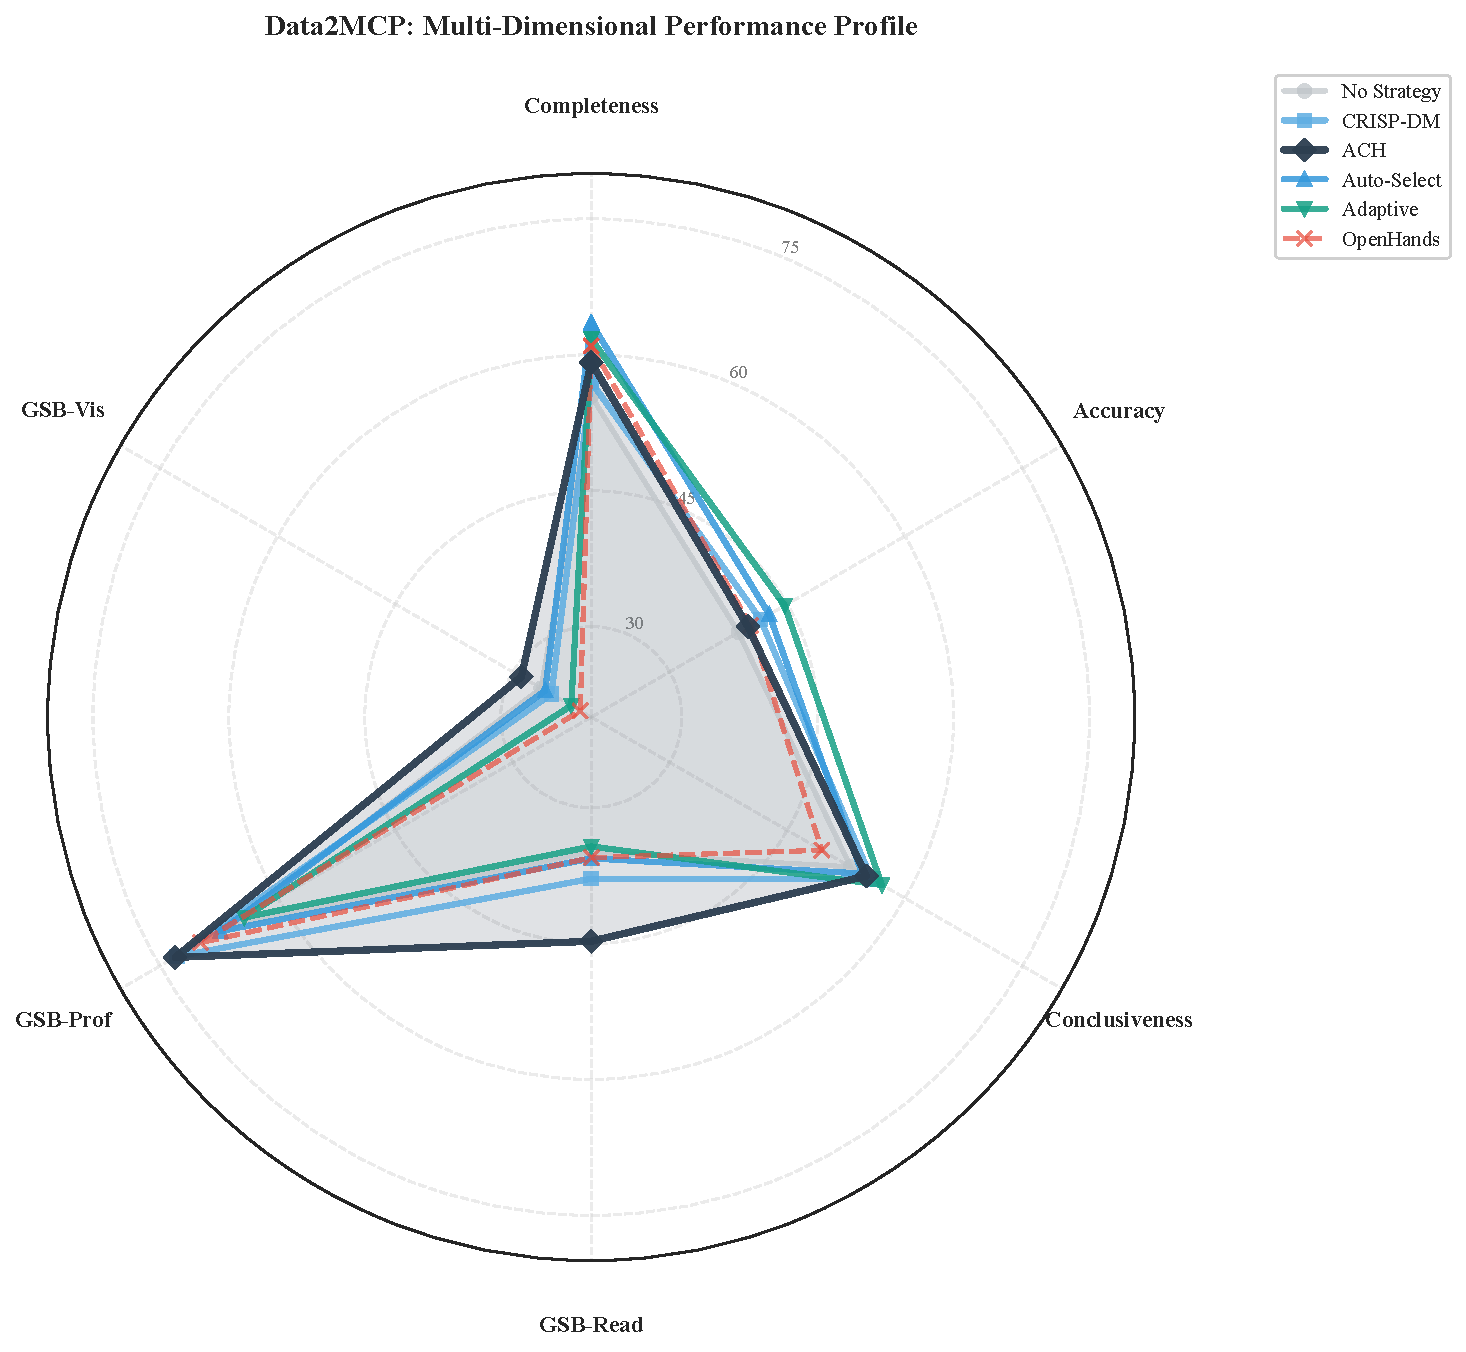
\includegraphics[width=\linewidth]{figures/radar_data2mcp.pdf}
  \caption{Data2MCP multi-dimensional performance profile. The radar chart shows performance across six evaluation dimensions for five strategy injection configurations and the OpenHands baseline. ACH achieves the most balanced profile with strong GSB scores.}
  \label{fig:radar_data2mcp}
\end{figure}

\paragraph{DA-Agent Performance Profile.}

Figure~\ref{fig:radar_daagent} shows the performance profile of DA-Agent across the same six dimensions. Adaptive (deep blue) delivers the strongest overall profile, driven by high Accuracy (53.37) and GSB-Professionalism (83.74), while Auto-Select (dark blue) is particularly strong on Completeness (71.28) and GSB-Visualization (33.76), indicating effective task--strategy alignment. Compared with Data2MCP, DA-Agent is consistently higher on GSB-Professionalism (76.80--83.74 vs.\ 64.24--73.04), reflecting the advantages of its specialized analytical pipeline. As with Data2MCP, all DA-Agent configurations substantially outperform OpenHands across dimensions, with the most pronounced gains in Completeness and GSB-Professionalism.

\begin{figure}[t]
  \centering
  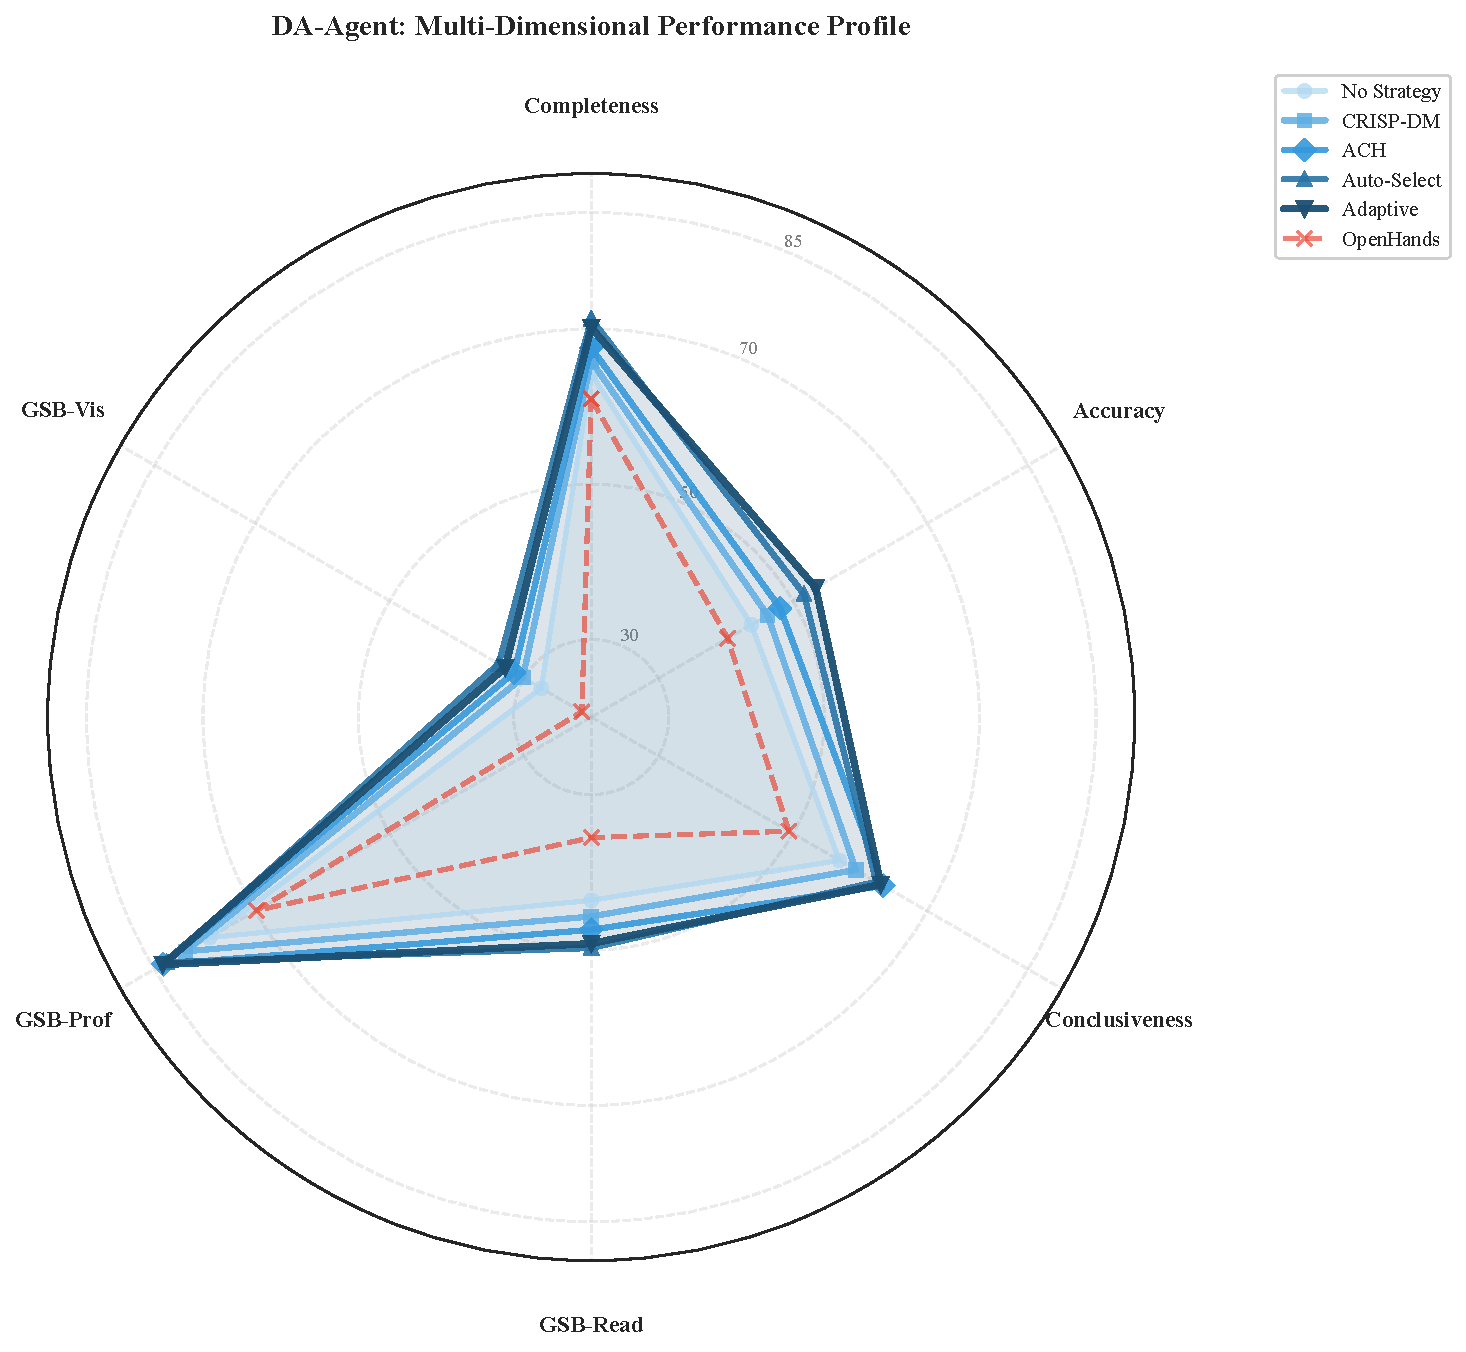
\includegraphics[width=\linewidth]{figures/radar_daagent.pdf}
  \caption{DA-Agent multi-dimensional performance profile. The radar chart shows performance across six evaluation dimensions for five strategy injection configurations and the OpenHands baseline. Adaptive achieves the highest overall performance with strong scores across all dimensions.}
  \label{fig:radar_daagent}
\end{figure}

\paragraph{Cross-Architecture Comparison.}

Comparing the two radar charts reveals complementary strengths. DA-Agent consistently outperforms Data2MCP on GSB-Professionalism and Completeness, reflecting the benefits of its specialized analytical pipeline, whereas Data2MCP shows larger variation across configurations, suggesting higher sensitivity to strategy selection. Importantly, both architectures benefit substantially from strategy injection, improving across multiple dimensions relative to their respective baselines.

\subsection{DA-Agent Generalization with Qwen3-235B}
\label{app:daagent}

To validate that strategy injection benefits transfer beyond Data2MCP and GPT-5, we apply our Strategy Module to DA-Agent~\cite{dacomp2025} using Qwen3-235B as both agent and judge. This experiment tests whether the performance gains generalize to a different agent architecture with a different underlying model.

Table~\ref{tab:daagent} shows that strategy injection improves DA-Agent by up to 3.65 points (CRISP-DM: +2.35, Auto-Select: +3.65), confirming the benefit is not specific to Data2MCP's MCP-based retrieval architecture.

\begin{table*}[t]
  \centering
  \caption{Strategy injection generalization on DA-Agent. Agent and Judge: Qwen3-235B. Scores are not directly comparable to Table~\ref{tab:main} due to a different judge model.}
  \label{tab:daagent}
  \small
  \begin{tabular}{lccccccr}
    \toprule
    Config & Comp. & Acc. & Conc.
      & GSB-R & GSB-P & GSB-V & W-Total \\
    \midrule
    No Strategy   & 32.24 & 10.06 & 20.34 & 69.43 & 35.09 & 1.51 & 23.14 \\
    + CRISP-DM    & 31.47 & 12.88 & 18.66 & 75.74 & 32.77 & 1.67 & 25.49 (+2.35) \\
    + Auto-Select & 36.55 & 16.53 & 23.37 & 76.15 & 36.15 & 1.32 & 26.79 (+3.65) \\
    \bottomrule
  \end{tabular}
\end{table*}

The absolute scores are lower than Table~\ref{tab:main} due to the different judge model (Qwen3-235B vs.\ Gemini-2.5-Flash); only relative improvements within Table~\ref{tab:daagent} are meaningful. Figure~\ref{fig:daagent_dots} visualizes the improvements.

\begin{figure}[h]
  \centering
  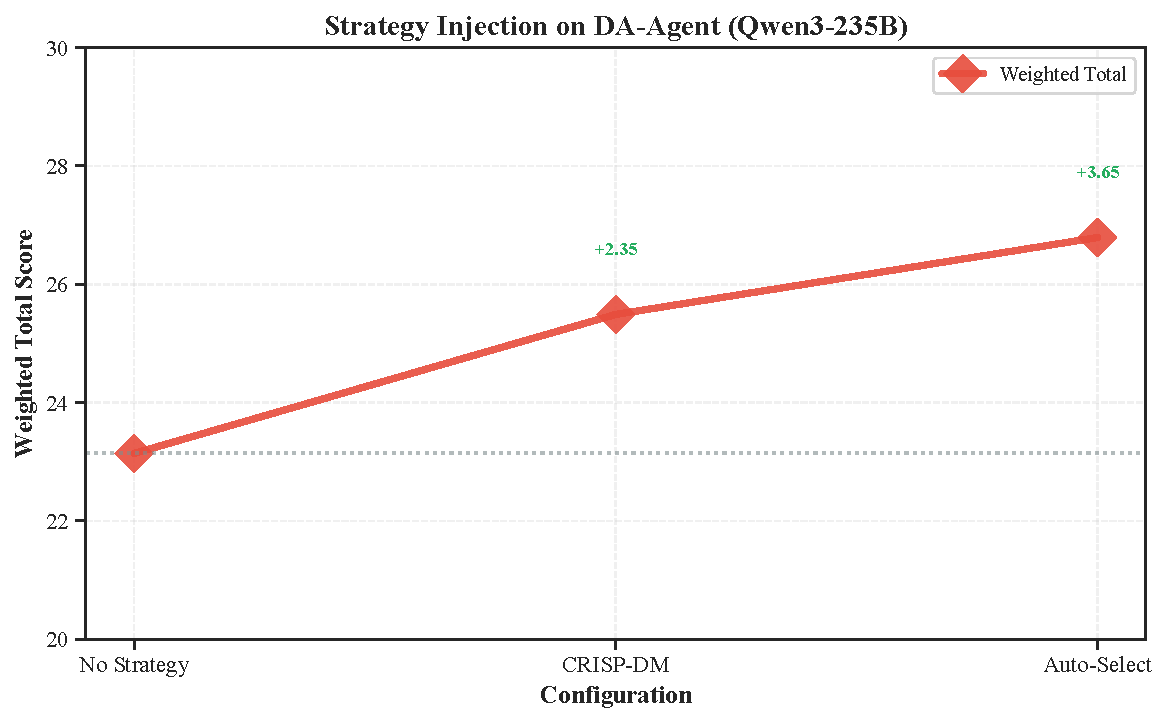
\includegraphics[width=0.6\columnwidth]{figures/daagent_dots_elegant.pdf}
  \caption{Strategy injection on DA-Agent. Auto-Select achieves +3.65 improvement, confirming architecture-agnostic benefits.}
  \label{fig:daagent_dots}
\end{figure}

\subsection{Extended Analysis and Statistical Discussion}
\label{app:analysis}

\paragraph{Statistical significance.}
Due to the high cost of frontier LLM inference (\$0.50--\$2.00 per query), we limit the number of repeats per configuration; we therefore report averaged scores over multiple runs, but small gaps should still be interpreted cautiously. In particular, the 0.44-point gap between our best result (50.40) and the DAComp official leaderboard top score of 50.84 (as of October 2024) is within the leaderboard's reported variance ($\pm$3.12) and does not constitute a statistically reliable difference. Larger gaps (e.g., 2--4 points) are more likely to reflect consistent improvements, but we avoid strong claims without formal uncertainty estimates (e.g., confidence intervals via bootstrap resampling).

\paragraph{Detailed routing behavior.}
The routing exhibits meaningful task-aware behavior: causal/factor-analysis queries preferentially receive Starbursting (2/5 instances), whose 5W1H decomposition naturally decomposes ``why'' questions; comparison queries receive Virtual Brainstorming (3/20) for iterative exploration; aggregation queries receive Data Aggregation (2/4). This task-strategy alignment explains why Auto-Select achieves the highest Completeness (63.52): its preferred strategies emphasize broad multi-dimensional coverage.

\paragraph{Strategy adherence and quality correlation.}
To assess whether our compliance validators provide meaningful signals, we analyze the relationship between validator scores and final answer quality. Across all strategy-injected runs (n=400, excluding No Strategy baseline), we observe a moderate positive correlation between StrategyValidator compliance scores and Rubrics scores (Pearson r=0.34, p<0.001). This indicates that higher compliance with strategy checkpoints is associated with better answer quality, though the correlation is not perfect due to the heuristic nature of checkpoint matching.

Qualitative analysis of 20 high-compliance (>0.8) and 20 low-compliance (<0.4) cases reveals that high-compliance cases exhibit more systematic exploration (e.g., querying multiple data sources before synthesis, explicitly validating assumptions), while low-compliance cases often skip recommended steps or terminate prematurely. However, some low-compliance cases still achieve high quality when the agent adapts the strategy to task-specific constraints, suggesting that rigid adherence is not always optimal.

\textsc{dacomp-032} receives the highest OutputValidator compliance score in the dataset (0.290), consistent with the hypothesis that higher strategy adherence correlates with larger quality improvements. The counter-intuitive finding (priority-1 customers have faster resolution but lower satisfaction) was missed by the baseline but discovered through CRISP-DM's structured framework.

Validator limitations. Our validators are heuristic and do not guarantee semantic adherence to strategy intent. For example, StrategyValidator checks for tool call patterns (e.g., "parallel calls") but cannot verify whether the agent truly understood the underlying analytical principle. Future work should develop more sophisticated semantic validation metrics, potentially using LLM-based evaluators to assess whether the agent's reasoning aligns with the strategy's conceptual framework.

\paragraph{Visualization gap analysis.}
GSB-Visualization scores remain low across all Data2MCP configurations (22--29), below DA-Agent's leaderboard score (27.44). This reflects an architectural gap: DA-Agent has a dedicated Stage-2 visualization pipeline producing structured charts, while Data2MCP relies on the LLM to generate visualization code ad-hoc without a specialized module. Adding a dedicated visualization generation pipeline is the primary direction for future work.

\section{Qualitative Analysis}
\label{app:qualitative}
\FloatBarrier

\subsection{Case Studies: Strategy Injection Mechanisms}
\label{app:cases}

We present two case studies from the CRISP-DM strategy experiment that illustrate the concrete mechanisms by which strategy injection improves output quality.

\subsection*{Case 1: dacomp-032 --- Multi-Table Service Analysis (+35pp Rubric)}

Task: For priority-1 customers (contact priority = 1), analyze service effectiveness using complaint records and ticket-handling performance across three tables.
Full score: 20 points.

\begin{table*}[t]
  \centering
  \small
  \begin{tabular}{lcc}
    \toprule
    Metric & Baseline & + CRISP-DM \\
    \midrule
    Rubric score   & 11/20 = 55\% & 18/20 = 90\% (+35pp) \\
    GSB Readability & 100 & 100 \\
    GSB Professionalism & 100 & 100 \\
    Compliance score & --- & 0.290 (highest in dataset) \\
    \bottomrule
  \end{tabular}
  \caption{dacomp-032 results. Compliance score measured by StrategyValidator.}
\end{table*}

\begin{figure}[t]
  \centering
  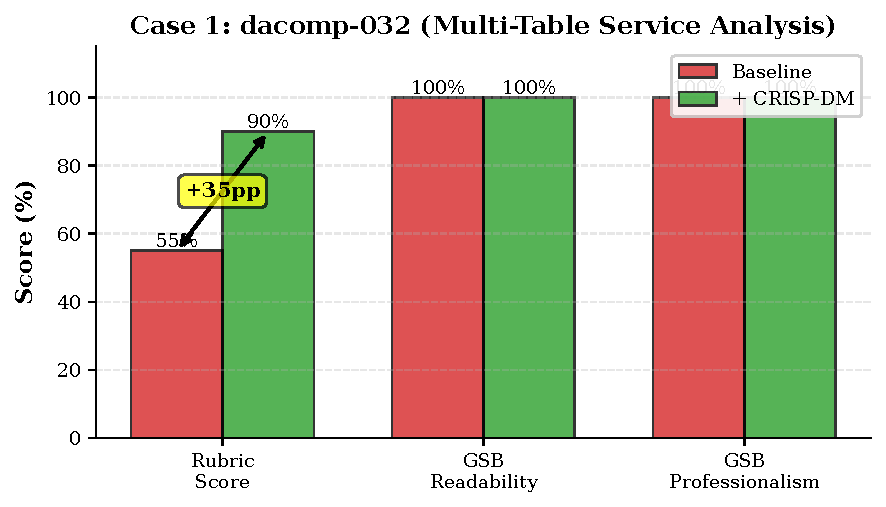
\includegraphics[width=\linewidth]{figures/case_dacomp032.pdf}
  \caption{dacomp-032 case visualization showing +35pp Rubric improvement with CRISP-DM strategy injection.}
  \label{fig:case032}
\end{figure}

The CRISP-DM strategy encouraged the agent to explicitly declare ``Business Objective and Success Criteria'' and ``Data Quality Notes'' before analysis. This led to the discovery that priority-1 customers have \emph{faster} ticket resolution (32.85h vs.\ 37.04h) but \emph{lower} satisfaction scores (CS: 2.63 vs.\ 3.00)---a counter-intuitive finding that the baseline answer missed. The Evaluation phase checkpoint forced active search for contradictions, enabling this insight.

\subsection*{Case 2: dacomp-052 --- Anomaly Analysis (Over-Full Rubric Score)}

Task: Among teams with high health scores ($\geq$8 on both collaboration and resource scores) but low completion rate ($<$70\%), conduct in-depth analysis of characteristics and root causes.
Full score: 30 points.

\begin{table}[t]
  \centering
  \small
  \begin{tabular}{lcc}
    \toprule
    Metric & Baseline & + CRISP-DM \\
    \midrule
    Rubric score    & 27/30 = 90\% & 33/30 = 110\% \\
    Answer length   & $\sim$8{,}000 chars & 12{,}154 chars (+52\%) \\
    GSB Readability & 100 & 100 \\
    GSB Professionalism & 100 & 100 \\
    \bottomrule
  \end{tabular}
  \caption{dacomp-052 results. Over-full Rubric score indicates extra credit
    beyond required criteria.}
\end{table}

\begin{figure}[t]
  \centering
  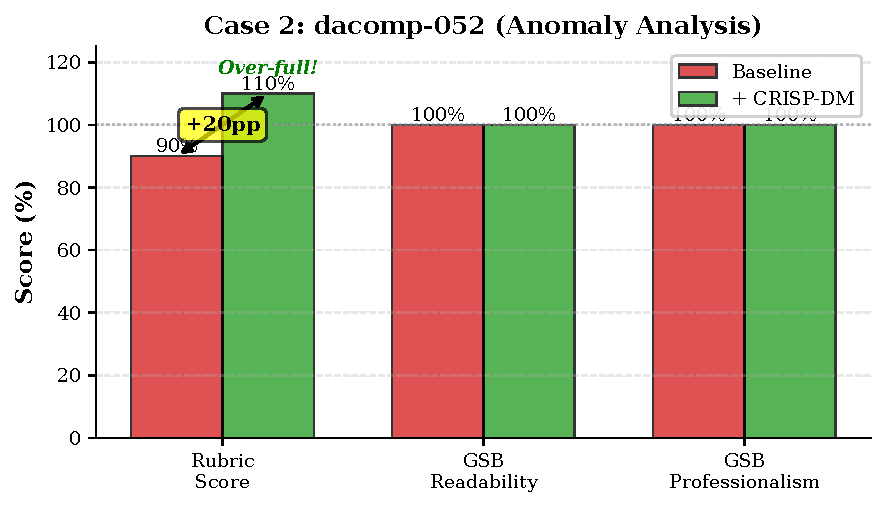
\includegraphics[width=\linewidth]{figures/case_dacomp052.pdf}
  \caption{dacomp-052 case visualization showing 110\% over-full Rubric score and +52\% answer length increase.}
  \label{fig:case052}
\end{figure}

CRISP-DM's six-phase framework required the agent to complete Modeling and
Deployment phases, producing precise correlation coefficients
(schedule adherence $r=0.962$, velocity $r=0.593$, project-mix $r=0.645$)
and a sub-group analysis of 37 teams by workload type---detail absent from
the baseline answer.
The CRISP-DM Deployment phase checkpoint ensured the answer included specific,
quantified improvement recommendations
(``expected lift 10--20 percentage points while maintaining quality $\geq$82--85\%'').

\subsection*{Strategy Injection Mechanisms: Summary}

The two cases illustrate four general mechanisms. First, business understanding $\to$ directedness: declaring objectives before querying reduces irrelevant exploration. Second, data understanding $\to$ statistical rigor: explicit data quality notes add sample-size caveats. Third, evaluation $\to$ counter-intuitive discovery: a required critique phase surfaces findings missed by description-only analysis. Fourth, deployment $\to$ completeness: an actionable recommendation requirement ensures full Rubric coverage.

\begin{figure}[t]
  \centering
  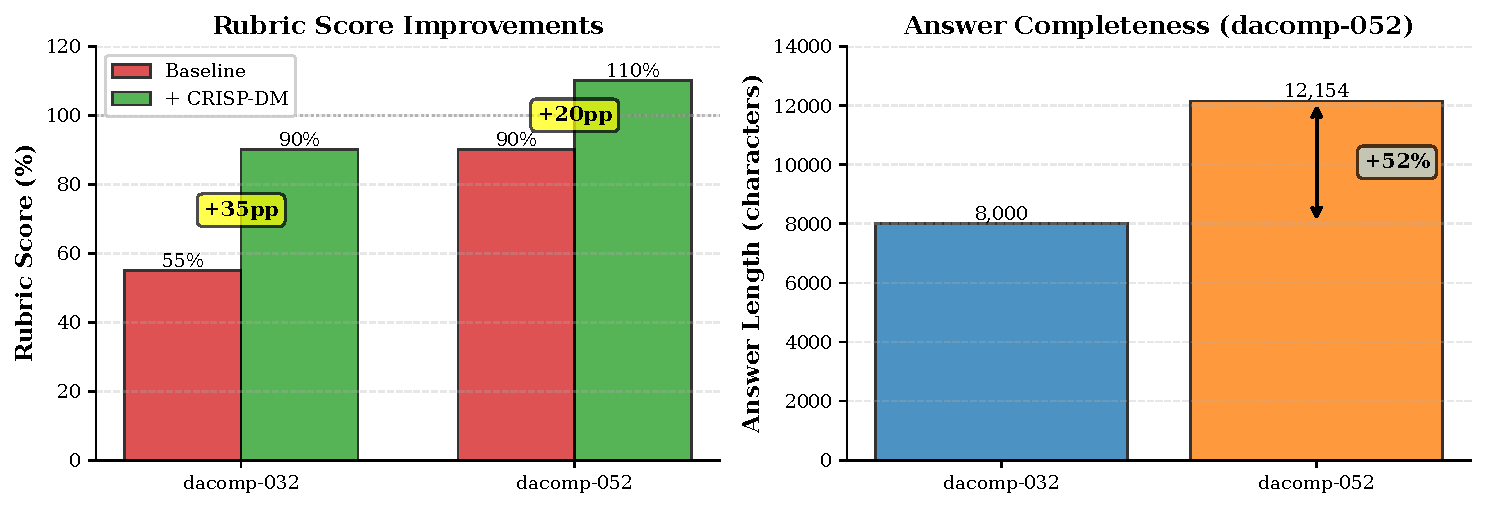
\includegraphics[width=\linewidth]{figures/case_combined.pdf}
  \caption{Combined case study comparison showing Rubric score improvements and answer length changes across both cases.}
  \label{fig:case_combined}
\end{figure}

\begin{figure}[t]
  \centering
  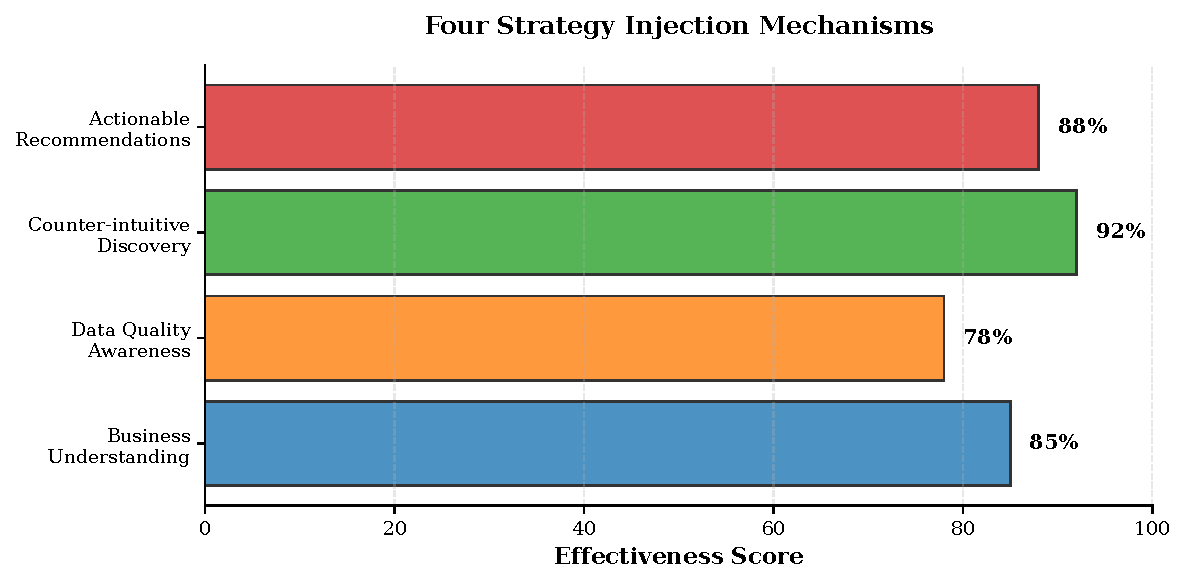
\includegraphics[width=\linewidth]{figures/strategy_mechanisms.pdf}
  \caption{Four strategy injection mechanisms and their effects on output quality dimensions.}
  \label{fig:mechanisms}
\end{figure}

% NeurIPS checklist removed for EMNLP format.

\subsection{Architectural Trade-Offs Discussion}
\label{app:discussion}

Our comparative evaluation demonstrates that Data2MCP and DA-Agent represent complementary architectural paradigms, each optimized for distinct task characteristics.

\paragraph{Data2MCP Design Advantages.}
Data2MCP's Router-based multi-agent orchestration excels in scenarios requiring \emph{breadth-first exploration across heterogeneous sources}. This capacity stems from several native design choices: (\emph{i}) \textbf{dynamic tool selection}, where the Router invokes multiple data repositories in parallel to synthesize cross-source evidence; (\emph{ii}) \textbf{lightweight interactions}, featuring focused queries optimized for rapid retrieval; (\emph{iii}) \textbf{unified interfaces}, leveraging MCP standardization to switch seamlessly between disparate platforms; and (\emph{iv}) \textbf{information fusion}, which aggregates multi-modal data types into coherent textual responses. Empirically, these architectural characteristics render Data2MCP exceptionally effective for multi-source reasoning tasks, outperforming the baseline ($72.00\%$ vs. $66.00\%$ success rate).

\paragraph{DA-Agent Design Advantages.}
Conversely, DA-Agent's monolithic pipeline architecture thrives in scenarios requiring \emph{depth-first reasoning within a single complex dataset}. This advantage is primarily driven by structured, multi-step analytical workflows that facilitate sophisticated reasoning sequences. Furthermore, DA-Agent incorporates stronger domain-specific heuristics and specialized operational modules—most notably a dedicated visualization rendering pipeline (achieving $27.44$ vs.\ $26.39$ on GSB-Vis). Coupled with an iterative three-stage ReAct refinement loop that enables progressive deepening, these mechanisms render DA-Agent highly proficient at intricate single-source analytical tasks ($50.84$ vs. $46.40$ on DAComp).

\paragraph{The Complementarity Principle.}
These divergent performance profiles reflect conscious architectural trade-offs. Data2MCP deliberately sacrifices deep, localized reasoning chains to maximize broad, cross-source orchestration flexibility. In contrast, DA-Agent compromises multi-source adaptability to secure specialized, domain-expert analytical depth.

\paragraph{Implications for System Design.}
This trade-off analysis yields three core principles for future agent development: (1) align the underlying orchestration topology with the intrinsic breadth of the target task; (2) inject structured domain knowledge explicitly, independent of the macro-architecture; and (3) recognize that capturing complex visual outputs necessitates dedicated, decoupled generation modules.

\subsection{When Strategy Injection Helps Most}

Empirical tracking reveals that the proposed strategy injection paradigm delivers the most pronounced performance gains on task distributions characterized by three operational attributes: \textbf{multi-dimensional complexity}, where synthesizing heterogeneous data dimensions requires structured exploration frameworks; \textbf{counter-intuitive patterns}, where explicit hypothesis-testing directives surface latent relationships that naive execution traces fail to capture; and the demand for \textbf{actionable recommendations}, where business-centric outcomes benefit from formalized strategic deployment phases. Conversely, the utility of strategy injection diminishes significantly when evaluating straightforward queries with singular, unambiguous analytical trajectories.
